%        File: pakapke-UML.tex
%   @author : pakpake
%     Created: mer. avril 22 10:00  2020 C
% Last Change: mer. avril 22 10:00  2020 C
%
\documentclass[a4paper,12pt]{article}

\usepackage[a4paper,margin=1in]{geometry}
\usepackage[utf8]{inputenc}
\usepackage[T1]{fontenc}
\usepackage{lmodern}
\usepackage[]{graphicx}
\usepackage{hyperref}
\usepackage[french]{babel}
\usepackage{xcolor}
\usepackage{minted}
\usepackage{caption}

\renewcommand{\listoflistingscaption}{Liste des codes}

%--\setlength{\parskip}{2ex}

\title{Programmation Objet Avancée \\ Examen UML}
\author{ }
\date{4 Mai 2020}

\begin{document}
\maketitle
\begin{abstract}
    Ce document est la synthèse du contrôle d'UML. Il comprend systématiquement les diagrammes demandés, tous réalisés avec le logiciel PlantUml. Les codes permettant de reproduire les figures sont donnés après chaque figure. Les codes sont exécutables en ligne sur le serveur de PlantUml à l'adresse suivante : \href{http://www.plantuml.com/plantuml/uml/}.
\end{abstract}

\tableofcontents
\clearpage
\listoffigures
\listoflistings
\clearpage

\section{Question 1}\label{question-1}

On distingue 3 cas d'utilisation :
\begin{itemize}
    \item Jouer une partie de démineur
    \item Configurer le jeu
    \item Consulter l'aide en ligne
\end{itemize}

L'objectif principal est de jouer une partie. Les 2 autres cas d'utilisation sont secondaires.
Ils auront donc la propriété <<\emph{extend}>>. On a donc le diagramme de cas d'utilisation représenté dans la figure~\ref{fig:utilisation} :


\begin{figure}[htbp]
    \centering
    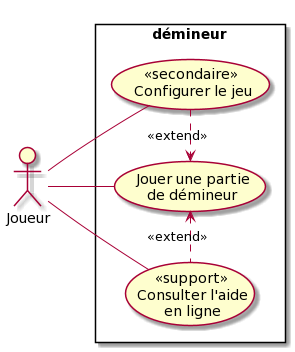
\includegraphics[width=.5\textwidth]{./images/q1.png}
    \caption{Diagramme de cas d'utilisation pour le jeu de démineur}
    \label{fig:utilisation}
\end{figure}

Dont voici le code réalisé grâce à \href{https://plantuml.com/}{PlantUml} donné dans le listing~\ref{listing:utilisation}

\begin{listing}[ht]
    \inputminted[bgcolor=lightgray!40,linenos=true]{fsharp}{./code-images/q1}
    \caption{Code du diagramme de cas d'utilisation}
    \label{listing:utilisation}
\end{listing}

\clearpage

\section{Question 2}\label{question-2}

\subsection{a)}\label{a}

Le but du jeu est de découvrir/démasquer ou marquer des cases sans tomber sur des mines. Le joueur ne va donc faire que cela jusqu'à ce qu'il gagne dans le meilleur des cas. S'il gagne, il aura donc fait un certain temps qui sera enregistré dans les meilleurs scores. Tout ceci peut être fait via une boucle (``loop'') grâce à laquelle le joueur à 2 choix réalisables dans n'importe quel sens grâce au bloc ``alt''.
Ce diagramme est présenté dans la figure~\ref{fig:seqa}.

\begin{figure}[htbp]
    \centering
    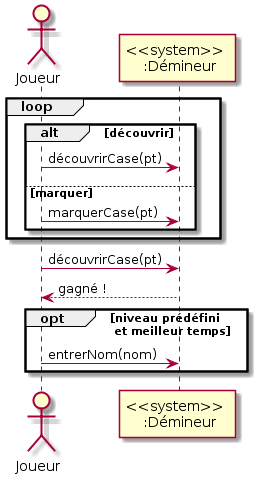
\includegraphics[width=.5\textwidth]{./images/q2-a.png}
    \caption{Diagramme de séquence}
    \label{fig:seqa}
\end{figure}


Ce diagramme n'est pas complet, il manque le cas où le joueur perd, et avant cela la configuration du jeu, comme par exemple le niveau de difficulté.

Le code de la figure~\ref{fig:seqa} en PLantUml est donné dans le listing~\ref{listing:seqa}.

\begin{listing}[ht]
    \inputminted[bgcolor=lightgray!40,linenos=true]{fsharp}{./code-images/q2-a}
    \caption{Code du diagramme de séquence}
    \label{listing:seqa}
\end{listing}

\clearpage

\subsection{b)}\label{b}

On ajoute à notre diagramme de séquence l'option permettant la configuration du jeu. Celle-ci est en amont de la séquence de jeu. Elle se place donc au dessus dans le diagramme de séquence.

\begin{figure}[htbp]
    \centering
    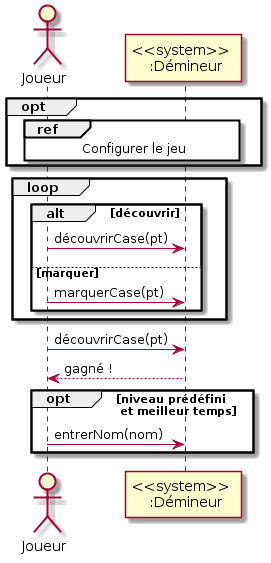
\includegraphics[width=.5\textwidth]{./images/q2-b.png}
    \caption{Diagramme de séquence avec configuration}
    \label{fig:seqb}
\end{figure}


Le code de la figure~\ref{fig:seqb} en PLantUml est donné dans le listing~\ref{listing:seqb}.

\begin{listing}[ht]
    \inputminted[bgcolor=lightgray!40,linenos=true]{fsharp}{./code-images/q2-b}
    \caption{Code du diagramme de séquence avec configuration}
    \label{listing:seqb}
\end{listing}

\clearpage

\subsection{c)}\label{c}

Et enfin, nous avons le diagramme final, qui prend bien en compte, le fait que le joueur puisse gagner ou perdre. Ceci est représenté avec l'opérateur ``break''.

\begin{figure}[htbp]
    \centering
    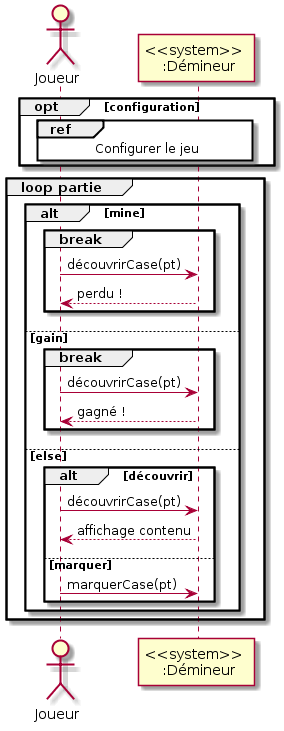
\includegraphics[width=.4\textwidth]{./images/q2-c.png}
    \caption{Diagramme de séquence complet}
    \label{fig:seqc}
\end{figure}

\clearpage

Le code de la figure~\ref{fig:seqc} en PLantUml est donné dans le listing~\ref{listing:seqc}.

\begin{listing}[ht]
    \inputminted[bgcolor=lightgray!40,linenos=true]{fsharp}{./code-images/q2-c}
    \caption{Code du diagramme de séquence complet}
    \label{listing:seqc}
\end{listing}

\clearpage

\section{Question 3}\label{question-3}

Le diagramme de classe d'analyse (voir figure~\ref{fig:analyse}) nous permet de représenter le jeu avec une configuration complète. C'est-à-dire le nombre minimal de mines, le nombre de mines restantes, le niveau de jeu, et le résultat. Mais aussi, la taille du plateau, le nom du joueur, le temps passé depuis le début de la partie, les coordonnées de la case et des ses voisines, et si la case est minée ou non.

\begin{figure}[htbp]
    \centering
    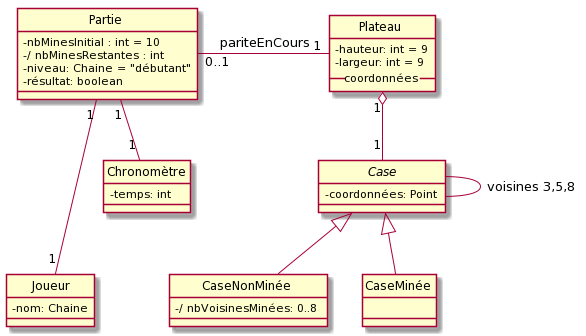
\includegraphics[width=1\textwidth]{./images/q3-Analyse.png}
    \caption{Diagramme de classe d'analyse}
    \label{fig:analyse}
\end{figure}


Le code de la figure~\ref{fig:analyse} en PLantUml est donné dans le listing~\ref{listing:analyse}.

\begin{listing}[ht]
    \inputminted[bgcolor=lightgray!40,linenos=true]{fsharp}{./code-images/q3-Analyse}
    \caption{Code du diagramme de classe d'analyse}
    \label{listing:analyse}
\end{listing}

\clearpage

Le diagramme d'état de la classe Case, nous permet quant à lui, de connaitre l'état de la case après l'action du joueur.
Ce diagramme est représenté dans la figure~\ref{fig:case}.

\begin{figure}[htbp]
    \centering
    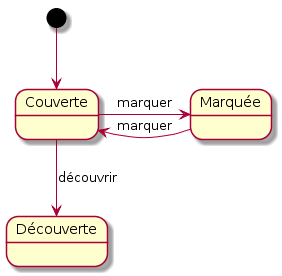
\includegraphics[width=.5\textwidth]{./images/q3-Case.png}
    \caption{Diagramme de classe d'analyse}
    \label{fig:case}
\end{figure}


Le code de la figure~\ref{fig:case} en PLantUml est donné dans le listing~\ref{listing:case}.

\begin{listing}[ht]
    \inputminted[bgcolor=lightgray!40,linenos=true]{fsharp}{./code-images/q3-Case}
    \caption{Code du diagramme d'état de la classe Case}
    \label{listing:case}
\end{listing}

\clearpage

\section{Question 4}\label{question-4}

Nous devons donc réaliser un diagramme de séquence, qui permet de représenter dynamiquement les échanges entre les différents objets et acteurs en fonction du temps.
Ici, ce diagramme (voir figure~\ref{fig:q4-1}) permet de représenter l'opération système \emph{marquerCase(pt)}, ce qui nous permet entre autre d'avoir une gestion presque complète des actions faites sur chaque case.

\begin{figure}[htbp]
    \centering
    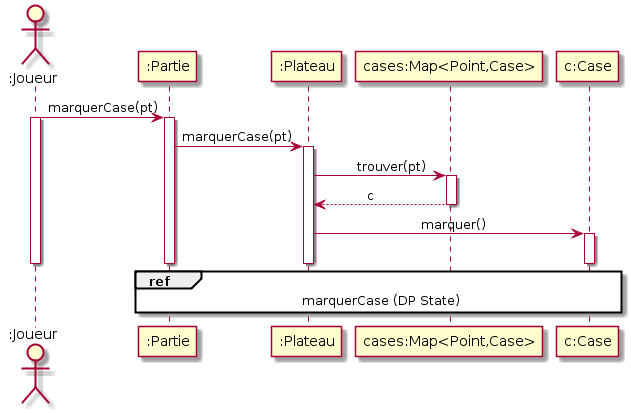
\includegraphics[width=1\textwidth]{./images/q4-1.png}
    \caption{Diagramme de séquence pour l'opération système \emph{marquerCase(pt)}}
    \label{fig:q4-1}
\end{figure}


Le code de la figure~\ref{fig:q4-1} en PLantUml est donné dans le listing~\ref{listing:q4-1}.

\begin{listing}[ht]
    \inputminted[bgcolor=lightgray!40,linenos=true]{fsharp}{./code-images/q4-1}
    \caption{Code du diagramme de séquence pour l'opération \emph{marquerCase(pt)}}
\end{listing}

\clearpage

Mais il faut l'améliorer, c'est pourquoi il y a un 2ème diagramme qui permet donc la gestion complète qui est faite à chaque action sur chaque case. Par exemple, décrémenter ou incrémenter le nombre de mines restante au cours de la partie, en fonction de l'état de la case, si elle est découverte, couverte ou bien marquée.

\begin{figure}[htbp]
    \centering
    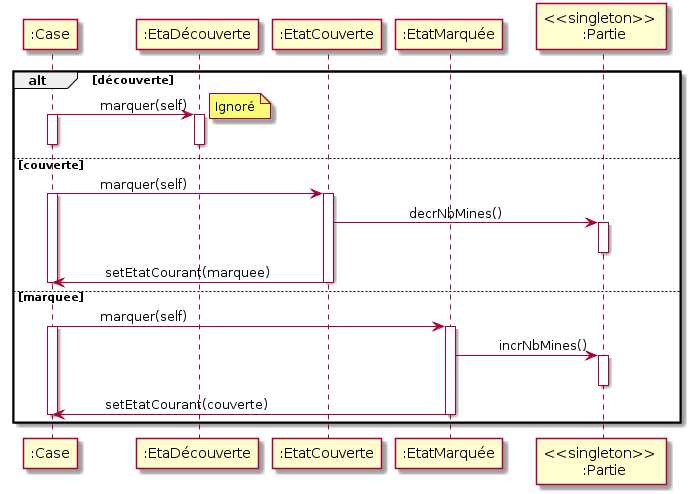
\includegraphics[width=1\textwidth]{./images/q4-2.png}
    \caption{Diagramme de séquence}
    \label{fig:q4-2}
\end{figure}


Le code de la figure~\ref{fig:q4-2} en PLantUml est donné dans le listing~\ref{listing:q4-2}.

\begin{listing}[ht]
    \inputminted[bgcolor=lightgray!40,linenos=true]{fsharp}{./code-images/q4-2}
    \caption{Code du diagramme de séquence}
    \label{listing:q4-2}
\end{listing}

\clearpage

\section{Question 5}\label{question-5}

Nous avons ici 3 diagrammes.

On se replace maintenant au niveau plus général avec le joueur, la partie, le plateau, la  collection des cases et une instance particulière de case.
Dans ce diagramme ``Partie'' délègue à ``Plateau'' l'action ``découvrirCase'' qui en s'adressant à la collection de cases va pouvoir savoir si une case est découverte.
L'action \emph{découvrirCase} est maintenant un groupe ``ref'' (\emph{Design Pattern State}).

\begin{figure}[htpb]
    \centering
    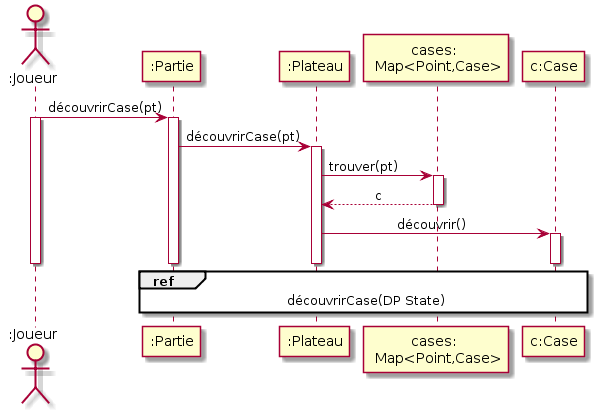
\includegraphics[width=1\textwidth]{./images/q5-1.png}
    \caption{Diagramme de séquence de conception pour \emph{découvrirCase(pt)}}
    \label{fig:q5-1}
\end{figure}

Le code de la figure~\ref{fig:q5-1} en PLantUml est donné dans le listing~\ref{listing:q5-1}.

\begin{listing}[ht]
    \inputminted[bgcolor=lightgray!40,linenos=true]{fsharp}{./code-images/q5-1}
    \caption{Code du diagramme de la séquence de conception pour \emph{découvrirCase(pt)}}
    \label{listing:q5-1}
\end{listing}

\clearpage

Le diagramme de la figure~\ref{fig:q5-2} est l'implémentation du groupe référence du diagramme de la figure~\ref{fig:q5-1}.
La situation ici a plus de conséquences car le fait de dévoiler une case dépend de son état (case avec une mine ou non) et cela pourrait soit interrompre le jeu, soit permettre de continuer la partie. Ainsi, l'opération ``dévoiler'' a plusieurs modes de fonctionnement qui dépendent de la situation du jeu. Le groupe référence \emph{dévoiler} est donc une opération polymorphe. Elle sera détaillée dans le diagramme de la figure~\ref{fig:q5-3}. 


\begin{figure}[htpb]
    \centering
    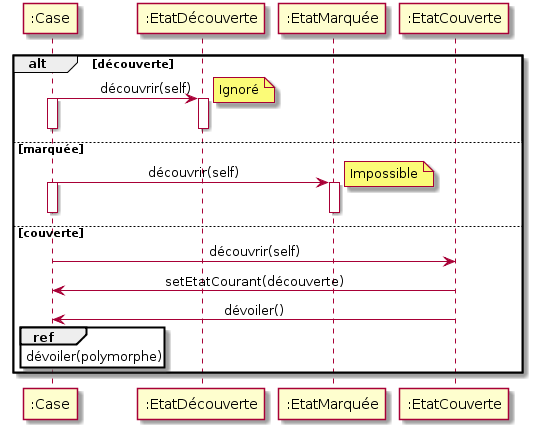
\includegraphics[width=1\textwidth]{./images/q5-2.png}
    \caption{Diagramme de séquence}
    \label{fig:q5-2}
\end{figure}

Le code de la figure~\ref{fig:q5-2} en PLantUml est donné dans le listing~\ref{listing:q5-2}.

\begin{listing}[ht]
    \inputminted[bgcolor=lightgray!40,linenos=true]{fsharp}{./code-images/q5-2}
    \caption{Code du diagramme de séquence}
    \label{listing:q5-2}
\end{listing}

\clearpage

Ce 3eme diagramme, détaille l'implémentation de l'opération \emph{dévoiler}.
Si la case contient une mine, alors on va enchaîner les actions suivantes :

\begin{itemize}
    \item arrêter le chronomètre
    \item découvrir toutes les mines non trouvées
    \item marquer avec un ``X'' les cases faussement marquées comme contenant une mine
\end{itemize}

Si la case ne contient pas de mine et est numérotée, alors il faut vérifier si la partie est gagnée ou non.

La dernière alternative est une case vide et dans ce cas, on lance l'opération \emph{découvrir} à toutes les cases voisines.

La figure~\ref{fig:q5-3} donne le diagramme de conception de l'opération polymorphe \emph{dévoiler}.

\begin{figure}[htpb]
    \centering
    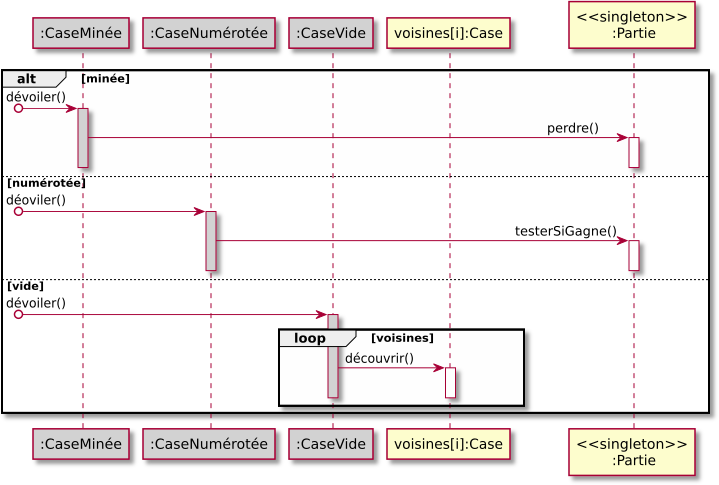
\includegraphics[width=1\textwidth]{./images/q5-3.png}
    \caption{Diagramme de séquence de l'opération polymorphe \emph{dévoiler}}
    \label{fig:q5-3}
\end{figure}

Le code de la figure~\ref{fig:q5-3} en PLantUml est donné dans le listing~\ref{listing:q5-3}.

\begin{listing}[ht]
    \inputminted[bgcolor=lightgray!40,linenos=true]{fsharp}{./code-images/q5-3}
    \caption{Code du diagramme de séquence de l'opération polymorphe \emph{dévoiler}}
    \label{listing:q5-3}
\end{listing}

\clearpage

\section{Question 6}\label{question-6}

En combinant toutes les opérations des diagrammes de séquence précédents dans les bonnes classes, on peut construire ce dernier diagramme de classe de conception du jeu de démineur. On peut apercevoir l'héritage de \emph{CaseMinée}, \emph{CaseVide}, \emph{CaseNumérotée} de \emph{Case} ainsi que l'héritage de \emph{EtatDécouverte}, \emph{EtatMarquée}, \emph{EtatCouverte} de \emph{EtatCase}.

Le diagramme est représenté dans la figure~\ref{fig:q6}.

\begin{figure}[htpb]
    \centering
    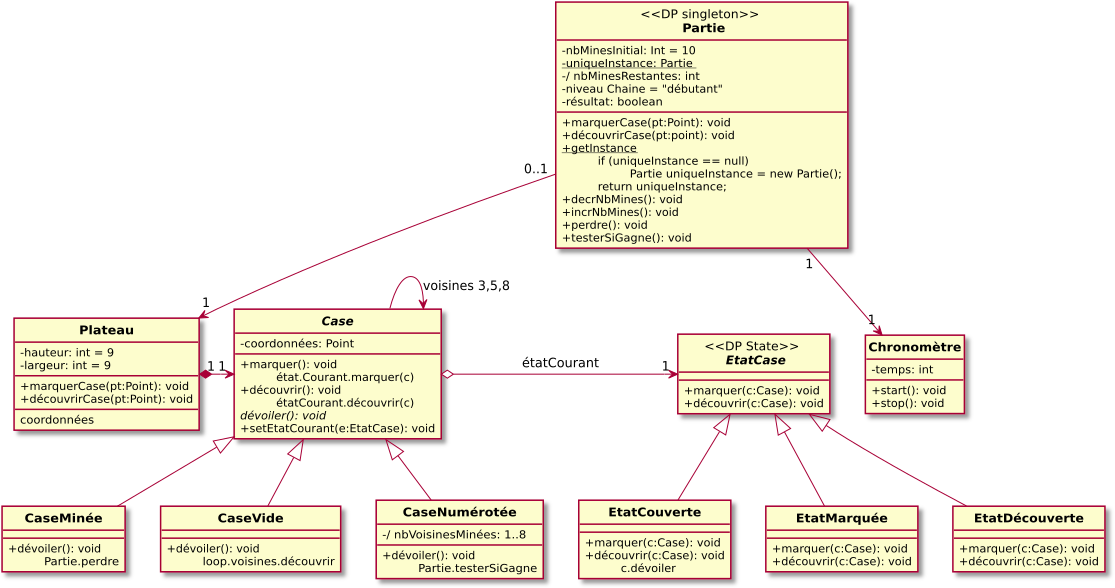
\includegraphics[width=0.74\textheight,angle=-90]{./images/q6-modif.png}
    \caption{Diagramme de classe de conception du jeu complet}
    \label{fig:q6}
\end{figure}

\clearpage

Le code de la figure~\ref{fig:q6} en PLantUml est donné dans le listing~\ref{listing:q6}.

\inputminted[bgcolor=lightgray!40,linenos=true]{fsharp}{./code-images/q6}
\captionof{listing}{Code du diagramme de classe de conception du jeu complet \label{listing:q6}}

\end{document}
